%TC:group tabular 0 1
\chapter{Literature review and methodology} % Main chapter title
\label{chapter2} % For referencing the chapter elsewhere, use \ref{Chapter1}

% Define some commands to keep the formatting separated from the content
\newcommand{\keyword}[1]{\textbf{#1}}
\newcommand{\tabhead}[1]{\textbf{#1}}
\newcommand{\code}[1]{\texttt{#1}}
\newcommand{\file}[1]{\texttt{\bfseries#1}}
\newcommand{\option}[1]{\texttt{\itshape#1}}

%----------------------------------------------------------------------------------------

There are four major components to this capstone: The dataset, model training, application of XAI techniques to the trained models and evaluating the effectiveness of these XAI techniques. I provide a literature review and describe the chosen methodology of these components below.

%----------------------------------------------------------------------------------------
%	SECTION 1
%----------------------------------------------------------------------------------------
\section{Dataset: The APP-350 Corpus}
\label{app350_corpus}
The APP-350 Corpus consists of 350 annotated Android app privacy policies. Each data practice ("practice") consists of a data type and a modality. A data type describes a certain behaviour of an app that can have privacy implications (e.g. collection of a phone's device identifier or sharing of its location with ad networks). There are two modalities: \texttt{PERFORMED} (i.e. a practice is explicitly described as being performed) and \texttt{NOT\_PERFORMED} (i.e. a practice is explicitly described as not being performed). Altogether, 57 different practices were annotated. As not all practices had sufficient numbers to train models of sufficient baseline performance, I focused on training models on the top 5 practices by frequency\footnote{The performance of the models of the top $n$ frequently occurring practices is later elaborated on in Chapter~\ref{chapter4}.}. The data types and modalities that are used for the rest of the capstone are provided in Table~\ref{tab:data_practices} and ~\ref{tab:modalities}.

\begin{table}[]
	\resizebox{\textwidth}{!}{%
	\begin{tabular}{|l|p{0.8\linewidth}|}
	\hline
	\textbf{Data Type}                 & \textbf{Description}                                                                                    \\ \hline
	Contact\_E\_Mail\_Address & Describes collection of the user's e-mail.                                          \\ \hline
	Identifier\_Cookie\_or\_similar\_Tech & Describes collection of the user's HTTP cookies, flash cookies, pixel tags, or similar identifiers. \\ \hline
	Identifier\_IP\_Address   & Describes collection of the user's IP address.                                      \\ \hline
	Location                  & Describes collection of the user's unspecified location data.                       \\ \hline
	\end{tabular}%
	}
	\caption{List of top 5 data practices and their descriptions.}
	\label{tab:data_practices}
\end{table}

\begin{table}[]
	\resizebox{\textwidth}{!}{%
	\begin{tabular}{|l|p{0.8\linewidth}|}
	\hline
	\textbf{Party}                 & \textbf{Description}                                                                                    \\ \hline
	1stParty & Describes collection of data from the user by the app publisher.                                          \\ \hline
	3rdParty & Describes collection of data from the user by ad networks, analytics services, or other third parties. \\ \hline
	\end{tabular}%
	}
	\caption{List of modalities.}
	\label{tab:modalities}
\end{table}

The APP-350 Corpus was annotated and used in a broader project to train machine learning models to conduct a privacy census of 1,035,853 Android apps (\cite{zimmeck2019}). The authors downloaded the data privacy policies of apps from the Play Store with more than 350 million installs (which totalled 247 apps) and 103 randomly selected apps with 5 million installs. In total, there were data privacy policies of 350 apps. All 350 policies were annotated by one of the authors, a lawyer with experience in data privacy law. To ensure reliability of annotations, 2 other law students were hired to double annotate 10\% of the corpus. With a mean of Krippendorff's $\alpha = 0.78$\footnote{Krippendorff's $\alpha$ is a measure of agreement, with $\alpha > 0.8$ indicating good agreement, $0.67 <= \alpha <= 0.8$ indicating fair agreement, and $\alpha < 0.67$ indicating doubtful agreement.}, the agreement between the annotations exceeded previous similar research.

Since the focus of this capstone is to assess XAI methods within a data privacy context, the APP-350 corpus was chosen as it contains real-world data privacy practices from the PlayStore apps. Training models and evaluating XAI techniques on this dataset would provide a realistic indication of their performance. APP-350 is also a labelled dataset, allowing supervised training which provides a better validation of model performance. 

\subsection{Data pre-processing}
The annotated privacy policies were originally in \texttt{.yml}, with one \texttt{.yml} file containing one app data privacy policy. Each data privacy policy is labelled at both the sentence and segment\footnote{A segment is similar to a paragraph.} level, but to limit the scope of this capstone I focus only on sentence level. The data was restructured from \texttt{.yml} to \texttt{.csv}.

\section{Text representations and classifiers}
\subsection{Literature review}
In NLP, text representations are methods that translate plain text to mathematical representations that can be understood by a computer. The easiest and most intuitive text representation is a purely count-based approach such as Bag-of-Words, where each word is represented by their frequency in the sentence. These can be categorised as sparse vector representations. However, they do not capture the semantic and syntactic differences of words (\cite{liu2020word}). More advanced dense vector representations such as GloVe (Global Vectors) are better able to capture these differences. Generally, these dense vector representations are created through unsupervised learning. Neural networks are trained to predict the target word given surrounding words(\cite{liu2020word}). However, to capture such semantic meaning requires more abstraction and further increases the opacity and decreases the interpretability of NLP models. Hence, there is an inverse relationship between performance / opacity and interpretability.  This is typically described as the "black-box" problem of AI: only the inputs and outputs to the system can be observed, but how the model derived the outputs from the inputs is not known (or at least not easily understood) because it is difficult to know exactly how the model is programmed (\cite{zednik2021}). In generating text representations of the APP-350 corpus, Zimmeck et al. used a union of Tf-IDF vectors and manually crafted features which were Boolean values indicating the presence or absence of frequently occurring keywords that occurred in each data practice.

Another component of a classifier is the model used to generate predictions. These models can be broadly categorised into classical machine learning models such as logistic regression and decision trees, and neural networks such as GPT. However, while neural networks are higher performing, if simpler models are able to produce reasonable performance, these simpler models should be used instead. Much depends on the complexity of the text corpus, and the engineering task that the models are made for. Classical models are much less complex and therefore more explainable than neural networks, and require much less data to train. For the APP-350 corpus, Zimmeck et al. used support vector machine for classification (SVCs) to achieve reasonable performance. Individual classifiers were then trained for every data practice. For all the classifications (except for four categories), they trained SVCs with a linear kernel and five-fold cross validation. For the four policy classifications, word-based rule classifiers were used instead because of the limited number of training data.

For the top 5 data practices that this capstone is concerned about, Zimmeck et al. were able to achieve F1 scores ranging from 77\% (Identifier Cookie 1st Party), 91\% (Contact Email Address 1st Party) to around 90\% for location related data practices\footnote{Not all the data practices were used in training ($n = 188$) and testing ($n = 100$) these classifiers, so there is no reference performance for some of the data practices that are used in this capstone.}.

\subsection{Methodology}
Given that the focus is on explainability, and in any case the APP-350 corpus is probably too limited to train neural networks\footnote{For example, BERT was trained on the whole Wikipedia (and more), while GPT-2, the second iteration of GPT, was trained on 45 terabytes of data.}, I focus only on training classical models for prediction in this capstone. Since sparse vector representations and classical models have performed well for the APP-350 corpus as seen above, I use SVCs and Tf-IDF. For the sake of comparison, I also use logistic regression and pre-trained GloVe embeddings.

The idea behind Tf-IDF is that words that are frequent in a document but rare across the rest of the corpus are more important in distinguishing the document from others. The Tf-IDF metric for a word in a document is calculated by multiplying two different metrics:

\begin{enumerate}
	\item Term frequency (TF) of a word in a document. This is the number of times the word appears in a document.
	\item Inverse document frequency (IDF) of the word across a set of documents. This is calculated by taking the total number of documents and dividing it by the number of documents that contain the specific word. This calculates the rarity of the term across all the documents. The closer the IDF of a word is to 0, the more common the word is.
\end{enumerate}

In comparison, GloVe as a dense vector representation is able to better model semantic differences mathematically in the following way: $\text{King} - \text{Man} + \text{Woman} = \text{Queen}$ (\cite{vector_differences_2015}). GloVe is an unsupervised learning algorithm for obtaining vector representations for words. The length-50 vectors used in this capstone are pre-trained using this algorithm on Wikipedia and news articles (\cite{pennington2014glove}). The main idea behind GloVe is to learn text representations by considering the statistics of words that occur together in a corpus. These statistics capture how frequently different pairs of words occur together in the text. GloVe builds a matrix from these statistics, where each element represents the number of times two words appear together in the same context. The matrix is then factorized into a product of two low-rank matrices, where each row in one of the matrices represents a vector representation of a word. This results in dense, fixed-size vector representations for each word in the corpus that encode their meaning and relationships with other words in the corpus.

In terms of tokenisation for this capstone, for both Tf-IDF and GloVe representations, text was lowercased and stop words were removed. No stemming and lemming was conducted. For Tf-IDF specifically, 1-gram to 4-grams were generated in the case of Tf-IDF. For GloVe, length 50 pre-trained vectors were used to tokenise individual words, and then averaged across all of the words to represent one document.

In terms of models for prediction, I use SVC with a linear kernel. SVC works by finding the a linear hyperplane in a high-dimensional space that separates the different classes of data points with the maximum margin of separation (Figure~\ref{fig:svc_viz}). The hyperplane functions as a decision boundary and the margin is the distance between the hyperplane and the nearest datapoints from each class. I also use scikitlearn's SGDClassifier that implements linear SVC using gradient descent, which is another optimisation method apart from a linear kernel. I also use logistic regression as a baseline classifier for its simplicity. Logistic regression predicts the probability of a multi-class target variable as a function of the input features. The sigmoid function is usually used to transform the linear combination of features into a probability value between 0 and 1 (Figure~\ref{fig:log_reg_viz}). While I also trained ensemble classifiers (AdaBoost, GradientBoost, Random Forest), the performance of these models were roughly the same or less than logistic regression and SVC. Hence, I excluded them from the capstone.


\begin{figure}[!ht]
	\centering
	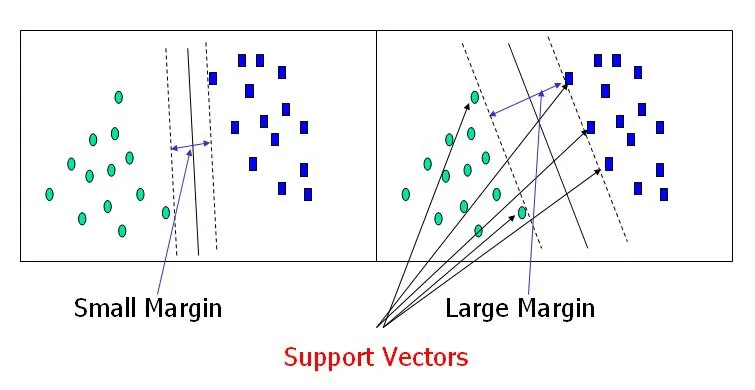
\includegraphics[width=1\linewidth]{figures/svc_viz.png}
	\caption{Finding the hyperplane in SVC (\cite{svc_viz}).}   
    \label{fig:svc_viz}
\end{figure}

\begin{figure}[!ht]
	\centering
	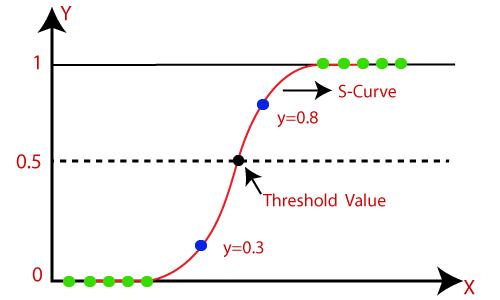
\includegraphics[width=1\linewidth]{figures/logistic_reg.png}
	\caption{Sigmoid function in logistic regression (\cite{log_reg_viz}).}   
    \label{fig:log_reg_viz}
\end{figure}


%-----------------------------------
%	SECTION 2
%-----------------------------------
\section{XAI methods for NLP}
\subsection{Literature review}
XAI for NLP have two broad characteristics: Local vs global, and self-explaining vs post-hoc. Thus, there are four possible categories of XAI as seen in Table~\ref{tab:xai_methods}.

\begin{table}[!ht]
	\resizebox{\textwidth}{!}{
	\begin{tabular}{|l|p{0.8\linewidth}|}
	\hline
	\textbf{Category}      & \textbf{Description}                                                                                                                            \\ \hline
	Local Post-Hoc         & Explain a single prediction by performing additional operations (after the model has made a prediction)                                         \\ \hline
	Local Self-Explaining  & Explain a single prediction using the model itself (calculated from information made available from the model as part of making the prediction) \\ \hline
	Global Post-Hoc        & Perform additional operations to explain the entire model's predictive reasoning                                                                \\ \hline
	Global Self-Explaining & Use the predictive model itself to explain the entire model's predictive reasoning                                                              \\ \hline
	\end{tabular}
	}
	\caption{The four categories of XAI for NLP, adapted from \cite{danilevsky2020}.}
	\label{tab:xai_methods}
	\end{table}

Some classical models such as logistic regression can be considered local and global self-explaining models. The coefficients of the features show the relative importance of each feature towards making the prediction. These coefficients are generated as part of the model training process and make it self-explaining. Logistic regression is also globally explainable since it models a deterministic function (sigmoid function), and this function serves as the "reason" for any prediction by the model. However, neural networks are not self-explaining by nature, in part as they are non-linear and are fitted onto high-dimensional data, in additional to the large numbers of parameters that make it difficult to ascertain the interaction between different features when a prediction is made. Therefore, post-hoc methods of explanability have to be used instead. 

\begin{figure}[!ht]
	\centering
	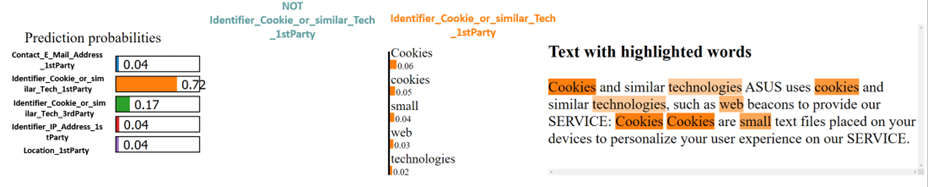
\includegraphics[width=1\linewidth]{figures/explanations_visualisations/section_4a/Picture1.png}
	\caption{Sample visualisation of LIME}   
    \label{fig:lime_sample}
\end{figure}

\subsection{Methodology}
I use LIME (Local Interpretable Model-agonistic Explanations), a local post-hoc XAI method that is also model agnostic (\cite{lime}). Given a trained NLP model, LIME generates a set of perturbations on the input sentence by randomly replacing some of the words with similar words. These perturbed samples are passed to the NLP model for prediction. Using these predictions, LIME fits a simple self-explaining model (such as a linear regression or a decision tree) to explain these predictions. Through this local self-explaining model, LIME is able to generate the contribution of each feature to a particular prediction for a single sample. Figure~\ref{fig:lime_sample} is an example of how an explanation of LIME can be visualised. Since LIME is a local, post-hoc method that uses a surrogate model to generate explanations, one disadvantage is that it may not fully represent how the underlying model actually made its prediction. Nevertheless, LIME has been found to be able to generate explanations that are faithful to the underlying model even just by using linear models for the surrogate model (\cite{lime}).

I chose to use LIME because it is model agnostic which allows easy experimentation with different combinations of text representations and models. Though logistic regression and SVC may be inherently self-explaining, I apply LIME on them because it visualises the feature importance without needing survey respondents to interpret coefficient scores of these models which can be inaccessible to those without a data science background. I apply LIME on the different combinations of text representations and models and compare the explainability of LIME's explanations. I presented these explanations to the survey respondents without any amendments to the code output, except for minor editing to the labels in the figure because some labels were cut-off.

\section{Evaluating the effectiveness of XAI methods}
\subsection{Literature review}
There is no consensus of the methods or standards of assessing XAI techiques (\cite{vilone2021}). Standards of explainability are highly dependent on the purpose of generating the explanations. A few purposes have been suggested (\cite{doshi-velez2017}):
\begin{enumerate}
	\item \textit{Global vs local:} A scientist inspecting a model predicting rainfall would require global explanation since he would be concerned with finding a long-term patterns, while a consumer who failed to obtain a loan would only require a local explanation to justify why the model made that specific decision.
	\item \textit{Area and severity of incompleteness of the problem:} A potential buyer of an autonomous vehicle (AV) would want a general overview of how AVs work, while a regulator may have specific explanation requirements such as whether a model detects a pedestrian 10 metres before collision.
	\item \textit{Nature of user expertise:} A layperson with no training in credit worthiness would not expect details of large complicated models in relation to the model's prediction of his credit rating, compared to an auditor that would expect explanations of comparable granularity and nuance as human auditors.
\end{enumerate}

Within the legal context, what could be insufficiently explainable for non-discrimination law (\cite{vale2022explainable}) might not apply \textit{mutatis mutandis} to the GDPR. In any case, this capstone makes no claim as to the applicable standard for explainability for data privacy, and merely serves as empirical insight as to the perceptions of explainability by potential data subjects.

In terms of methods of assessing XAI, human evaluation has been frequently utilised. (\cite{danilevsky2020}). This involves asking humans to evaluate the effectiveness of the explanations in various ways (Table~\ref{tab:human_eval_xai}). The metrics being evaluated include fidelity (how much the explanation reflects the actual workings of the model), comprehensibility (how easily understood are the explanations), and others. However, many studies also do not state what is being evaluated. 

\begin{table}[!ht]
	\resizebox{\textwidth}{!}{%
	\begin{tabular}{|p{0.2\linewidth}|p{0.85\linewidth}|}
	\hline
	\textbf{Method}                 & \textbf{Description}                                                                                                                                        \\ \hline
	Binary forced choice            & Humans are presented with pairs of explanation, and must choose the one that they find of higher quality.                                                   \\ \hline
	Forward simulation / prediction & Humans are presented with an explanation and an input, and must correctly simulate the model's output.                                                      \\ \hline
	Counterfactual simulation       & Humans are presented with an explanation, an input, and an output, and are asked what must be changed to change the model's prediction to a desired output. \\ \hline
	\end{tabular}
	}
	\caption{Methods of measuring human evaluation of XAI (\cite{doshi-velez2017}).}
	\label{tab:human_eval_xai}
\end{table}

Human evaluation has been conducted within a legal context (\cite{gorski2021}). The authors trained a CNN on a dataset that contained 50 decisions issued by the Board of Veterans' Appeals of the US Department of Veterans Affairs. Each sentence was annotated according to a type of legal reasoning (e.g. fact finding, legal reasoning, application of legal rule etc.). The focus of the research was to evaluate different XAI methods and lawyers' perceptions and expectations of XAI. Lawyers were asked to rate different XAI visualisations of the same 6 correctly classified sentences on a scale from 0 (worst) to 10 (best). Further, the lawyers that were surveyed were generally optimistic about the use of AI in law, with most agreeing that the explanations generated should be supplemented by further background knowledge, and that the model should be fair, lack bias, transparent and have awareness of the consequences of the AI-assisted / AI-automated decision. Lawyers also agreed that AI should increase automation and reduce their manual effort. 

In addition, there is no agreed upon definition of "explainability". Explainability could be influenced by other value-laden terms, such as, \textit{inter alia}, trust, effectiveness, fairness, bias, and the consequence of making a wrong prediction (\cite{rosenfeld2021}). The relative importance of these values and overall requirement of explainability is necessarily dependent on the purpose and user of the explanation. Values such as fairness, bias, risk and trust could be argued to be of specific importance in a legal context which includes data privacy. The notion of "rule of law" encompasses these values and legal systems are judged according to such values (\cite{greenstein2022}). Nevertheless, there is no definitive position as to how these values can be used to evaluate XAI techniques that are specifically used within a legal context.

\subsection{Methodology}
With the foregoing discussion in mind, I expand upon and tweak the methodology of Gorski and Ramakrishna. The primary method of evaluating LIME in this capstone is human evaluation through a survey. The survey was designed containing the following parts\footnote{The full survey can be found \href{https://github.com/TristanKoh/capstone-repo/blob/448263a933ae787027298e266f9202e7b3077524/survey/survey_questions.pdf}{here}, and a summary of the responses can be found \href{https://github.com/TristanKoh/capstone-repo/blob/448263a933ae787027298e266f9202e7b3077524/survey/survey_responses.pdf}{here}.}:
\begin{enumerate}
	\item \textbf{Demographic data and beliefs relating to data privacy and AI.} Respondents were asked to provide their major or subject area expertise if they had graduated. This is used as a proxy for their level of expertise in AI or data science. Respondents are also asked to rate how much they think AI is useful, is a risk as well as how far they are concerned about their data privacy. This is used to understand the respondents' beliefs such that their assessment of LIME and the models can be evaluated in the context of these beliefs. Further cross-sectional analysis of the survey data can also be conducted using these data.
	\item \textbf{Rating of explainability metrics from the perspectives of three stakeholders in data privacy.} After a brief explanation of the data practices and how NLP works, respondents were provided with three contexts (app developer, PDPC \& user) to measure the variability of different values related to explainability across different purposes of explanation. All three contexts relate to using the classifier to make a decision with legal consequences, and are meant to vary the purposes of the explanation according to the three purposes suggested by Doshi-Velez \& Kim above. After reading each context, the respondents are required to rate their beliefs relating to the use of the classifier in that particular context across four metrics: Effectiveness of model, Fairness, Risk to society, and trust in the model. These metrics were chosen as they are values of importance specifically to a legal decision making context, and are used to measure how these values that relate to explainability can vary according to the purposes of the explanation. 
	\item \textbf{Rating of the LIME visualisations of four classifications by the same classifier (Logistic regression + Tf-IDF).} Respondents were asked to rate how far they understood why the model made the prediction, and how far they found the visualisation easy to interpret. The intent is to evaluate both the underlying XAI technique (LIME) and the visualisation of the technique. For three classifications, respondents were given a counterfactual sentence replaced with words that were considered important by the classifier, and asked to predict whether the sentence would be classified under \texttt{Identifier Cookie 1st Party}. Counterfactual simulation is meant to provide another metric to measure explainability, aside from self-reported scores.
	\item \textbf{Choosing the more interpretable visualisation from a pair of identically classified sentences.} This uses binary forced choice to evaluate which text representation and model are more interpretable. Part 4 presents 3 pairs of visualisations from SVC + GloVe and Logistic regression + GloVe (controlling for text representation) and Part 5 presents another 3 pairs of visualisations from SVC + Tf-IDF and SVC + GloVe (controlling for model). Respondents were not told that the visualisations were produced by different models or text representations. The respondents' choices are then totalled up and compared against traditional performance metrics (P/R/F1) of the classifiers, to investigate whether there is a relation between interpretability and model performance.
	\item \textbf{Repeating the questions for the same three contexts.} Respondents are asked to view the same three contexts and answer the same questions in Part 2. This evaluates whether viewing the explanations significantly changed the respondents' beliefs according to the four metrics, and whether there are intra-relations and trends of the individual metrics and contexts.
\end{enumerate}

The survey was hosted on Google Forms, and respondents were recruited through friends and acquaintances of this author. The only restriction on recruitment was an age requirement of 18 and over for NUS / Yale-NUS students, or 21 and over for the general public due to Yale-NUS Ethics requirements.